\vspace*{-1mm}

This chapter focuses on the setup and the calibration of the $\CC$s in the SPS for the 2018 tests. The objective is to provide a full understanding of the operational aspects of the $\CC$s in the SPS and clarify the measurement of the $\CC$ voltage. 

The presented studies were performed by the author in addition to the first round of analysis in 2018. They were motivated by the results of the experimental campaign (Chapter~\ref{Ch:2018_analyisis}), which appeared to differ significantly from the theoretical predictions without apparent reason.
As the reason for that discrepancy was not understood, having a closer look and reviewing the procedure of the $\CC$ voltage calibration was essential, given that it is one of the most crucial parameters for the emittance growth studies (see Chapter~\ref{Ch:CC_noise_theory}, Eq.~\eqref{eq:dey_an} and Eq.~\eqref{eq:dey_pn}). 

%In 2018 the $\CC$ technology was tested with proton beams in the SPS for the first time. In this chapter, the setup and the calibration of the $\CC$s in the SPS are presented along with the demonstration of the first crabbings of proton beams. The objective is to provide a full understanding of the operational aspects of the $\CC$s in the SPS and clarify the measurement of the $\CC$ voltage which is one of the most crucial parameters for the emittance growth studies (see Chapter~\ref{Ch:CC_noise_theory}, Eq.~\eqref{eq:dey_an} and Eq.~\eqref{eq:dey_pn}). These studies, were performed by the author in addition to the first round of analaysis in 2018 motivated by the experimental results that will be presented later (Chapter~\ref{Ch:2018_analyisis}).

The chapter is structured as follows: Section~\ref{sec:cc_sps_installation} describes the installation of the $\CC$ system in the SPS. Thereafter, Section~\ref{sec:CC_operational_considerations} elaborates on details for their operation in the SPS machine. In Section~\ref{sec:HT_info}, the use of the Head-Tail (HT) monitor as the main diagnostic in the $\CC$ tests is discussed, focusing on the reconstruction of the $\CC$ voltage from its reading. Last, Section~\ref{sec:CC_voltage_meas} provides a characterisation of the beam based $\CC$ voltage measurement and defines the voltage amplitude and its uncertainty.

\section{Crab Cavities' installation in the SPS}\label{sec:cc_sps_installation}
For the SPS tests two prototype $\CC$s of the Double Quarter Wave (DQW) type, which will be referred to as $\CC$1 and $\CC2$ throught this thesis, were fabricated by CERN and were assembled in the same cryomodule, shown in Fig.~\ref{fig:DQW_cryomodule}~\cite{Zanoni:2017}. For its installation an available space was found at the SPS Long Straight Section 6 (SPS-LSS6) zone. As this section is also used for the extraction of the beam to the LHC, the cryomodule was placed on a mobile transfer table~\cite{Calaga:2649807} which  moved the cryomodule in the beamline for the $\CC$ tests and out of it for the usual SPS operation without breaking the vaccum.

\begin{figure}[h]
   \centering         
   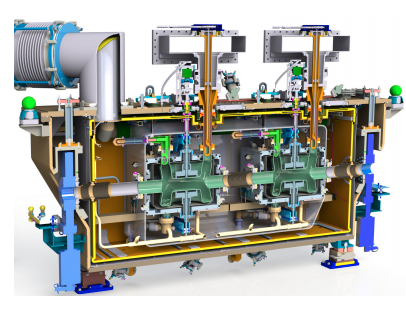
\includegraphics[width=0.8\textwidth]{images/Ch4/CC_cryomodule.png}
       \caption{Cross section view of the CC cryomodule~\cite{Zanoni:2017}. It has a total length of 3\,m~\cite{Baudrenghien:1520896} and at its core there are the two DQW cavities, which are illustrated with light green color.}
       \label{fig:DQW_cryomodule}
\end{figure}
% Couldn't find information on height, weight etc. Any idead where to look for spces?

% Photos from the cryomodule installation day: 1. https://home.cern/news/news/engineering/crabs-settled-tunnel (maybe good to show the scale?)
% 2. https://science.osti.gov/-/media/np/pdf/research/NP-Accel-RD-PI-Meeting/2019/Wu_2019FOA_PImeeting_crabcavity_Rev9.pdf?la=en&hash=B29283EDB3C704EC3EFD9DA23CA8DEA22076C88B

The main $\CC$s parameters are listed in Table~\ref{tab:SPS_CC_main}. Their location along the SPS ring is also indicated, in case someone would like to repeat the analysis described in this thesis.

\begin{table}[!hbt]
   \begin{minipage}{\textwidth}
   %\centering
   \begin{centering}
   \caption{Crab Cavities design parameters for the SPS tests in 2018.}
   \begin{tabu} to \textwidth {X[c,0.1m] X[c,m] X[0.5c,m] X[0.5c,m]}
		&&& \\[-6mm]
		\toprule \toprule
		\multicolumn{2}{l}{\textbf{Parameter}} &
		\multicolumn{2}{c}{\textbf{Value}} \\
		\bottomrule
      \multicolumn{2}{l}{} & 	\multicolumn{1}{c}{\textbf{CC1}} & \multicolumn{1}{c}{\textbf{CC2}} \\
      \midrule
      \multicolumn{2}{l}{crabbing plane}  & \multicolumn{1}{c}{vertical} & \multicolumn{1}{c}{vertical} \\
      
      \multicolumn{2}{l}{s-location$^{\ast}$}  & \multicolumn{1}{c}{6312.72\,m} & \multicolumn{1}{c}{6313.32\,m} \\

      \multicolumn{2}{l}{$\CC$ voltage, $\VCC$}  & \multicolumn{1}{c}{$\leq$ 3.4\,MV} & \multicolumn{1}{c}{$\leq$ 3.4\,MV} \\

      \multicolumn{2}{l}{$\CC$ frequency, $\fCC$}  & \multicolumn{1}{c}{400.78\,MHz} & \multicolumn{1}{c}{400.78\,MHz} \\ %400.789

      \multicolumn{2}{l}{Horizontal / Vertical beta function, $\beta_{x, CC}$ / $\beta_{y, CC}$}  & \multicolumn{1}{c}{29.24\,m / 76.07\,m} & \multicolumn{1}{c}{30.31\,m / 73.82\,m} \\

      \multicolumn{2}{l}{Horizontal / Vertical alpha function, $\alpha_{x, CC}$ / $\alpha_{y, CC}$} & \multicolumn{1}{c}{-0.88\,m / 1.9\,m} & \multicolumn{1}{c}{-0.91\,m / 1.86\,m} \\

      \multicolumn{2}{l}{Horizontal / Vertical dispersion, $D_{x, CC}$ / $D_{y, CC}$} & \multicolumn{1}{c}{-0.48\,m / 0\,m}  & \multicolumn{1}{c}{-0.5\,m / 0\,m} \\
      \arrayrulecolor{black}\bottomrule
	\end{tabu}
   \label{tab:SPS_CC_main}
   \end{centering} \footnotesize{$^\ast$ The s-location is reffered to the location of the elements along the SPS ring with respect to the start of the lattice i.e. element QF.10010 which is a focusing quadrupole. The s-location is given to allow the studies to be reproduced.}
   \end{minipage}
\end{table}
% QF.10010  is the start of the SPS lattice --> https://layout.cern.ch/reports/mad?fileType=STANDARD&machineId=2180065&versionId=34464591 (access with sshuttle)
% The actual start of the lattice at 0 m is: %BEGI.10010. which is a marker (not a real element).

% Optics parameters for CC and diagnostics in 2018: https://cernbox.cern.ch/index.php/apps/files/?dir=/__myshares/SPS_MDs_2018%20(id%3A271128)/SPSMeasurementTools&#editor

\section{Operational considerations}\label{sec:CC_operational_considerations}

For the beam tests with $\CC$s in the SPS the approach regarding the energy ramp and the adjustment of the phasing with the main RF system needed to be evaluated and they are briefly discussed here.

\normalsize{\textbf{Energy ramp}}\\
SPS receives the proton beam at 26\,GeV from the PS. It was found that the ramp to higher energies could not be performed with the $\CC$ on, as the beam was getting lost while crossing one of the vertical betatron sidebands due to resonant excitation~\cite{BE_seminar, CC_rephasing_RF}. Therefore, it was established that the acceleration has to be performed with the $\CC$ off and its voltage must be set up only after the energy of interest has been achieved. It is worth noting that this approach will also be used in the HL-LHC.

\normalsize{\textbf{Crab Cavity - main SPS RF synchronisation}}\\
It was important to ensure that during the "coast" the beam will experience the same kick from the $\CC$ each turn. In other words the SPS main RF system operating at 200\,MHz needed to be synchronous with the $\CC$ operating at 400\,MHz. Due to the larger bandwidth of the SPS main RF system the $\CC$ was used as a master. Therefore the $\CC$ was operating at a fixed frequency and phase, while the main accelerating cavities were adjusted to the exact half of the $\CC$ frequency and were re-phased so that they become synchronous with the crabbing signal. For the studies at higher energies the synchronisation took place at the end of the ramp shortly after the cavity was switched on~\cite{BE_seminar}.

% Steps for synchronisation: 1) SPS main RF was set at the exact half of the main RF. 2) The phase was adjusted. 3) The frequency needed to be re-adjusted slightly again such is it becomes the exact half of it.
% Nice explanation of the synchronisatio: https://journals.aps.org/prab/pdf/10.1103/PhysRevAccelBeams.24.062001
% For studies at the injection energy of 26\,GeV this synchronisation took place shortly after the injection. 


% Plotting figures in this section: /eos/user/n/natriant/2021/CC_MD_2021_summary/2018_HT_monitor
\section{SPS Head-Tail monitor as the main diagnostic}\label{sec:HT_info}
% info on the bandwidth of HT monitor https://indico.cern.ch/event/1044711/contributions/4389270/attachments/2264278/3844129/CCNoise_SPS_MDs.pdf

The SPS is equipped with a high bandwidth pick-up of approximately 2\,GHz allowing to resolve the intra-bunch motion. This instrument is called Head-Tail (HT) monitor and was originally designed for measuring chromaticity and transverse instabilities. However, in the SPS $\CC$ tests, the HT monitor was the main diagnostic device deployed for the demonstration of the crabbing and the measurement of the $\CC$ voltage (explained in details in Section~\ref{sec:CC_voltage_meas}). Therefore its use as a crabbing diagnostic should be explained here. The methods and procedures described in this section were developed at CERN and they are described here for the completeness of the thesis.

 In the first part of this section some general information on the instrument along with example signals will be presented. Subsequently, the post processing of the HT signal in the presence of the $\CC$ will be discussed. Last, the calibration of the $\CC$ voltage from the HT data is described and the visualisation of the crabbing is displayed. The experimental data presented in this section were acquired, on May 30, 2018 (time-stamp: 13:51:05), at the SPS injection energy of 26\,GeV with only one $\CC$, $\CC$1, at phase $\phiCC=0$ (this means that the particle at the center of the bunch doesn't recieve any transverse deflection) for simplicity. That energy of 26\,GeV was chosen to provide a better understanding of the methods used as the orbit shift from the $\CC$ kick is stronger and thus more visible than at higher energies.

% Post processing: /eos/user/n/natriant/2018/CC_MD_2018_summary/2018_HT_monitor/MD2_phase_scan_CC1/main_example_135105/plot_1example_HT_acquisition_for_thesis_30May2018-135105_for_thesis_sin_fit_forCh4_fixed_fcc.ipynb
\subsection{General information}\label{subsec:HT_general_info}
As already mentioned, the HT monitor is a high bandwidth version of a standard beam position monitor, which means that it can measure the transverse displacement within the bunch. This makes it ideal for the measurement of the intra-bunch offset caused from the $\CC$ kick. Its reading consists of the sum ($\Sigma$) and the  difference ($\Delta$) of the electrode signals of a straight stripline coupler (Fig.~\ref{fig:SPS_HT_diagram})~\cite{Jones:987561, Levens:2313358} over a defined acquisition period. The sum signal is the longitudinal line density while the difference signal corresponds to the intra-bunch offset. The system operates on timescales such that the signals are given as a function of the position within the bunch.

\begin{figure}[h]% Edit figure in: Goodle Docs/Doctoral/2022/Thesis/Ch4
   \centering         
   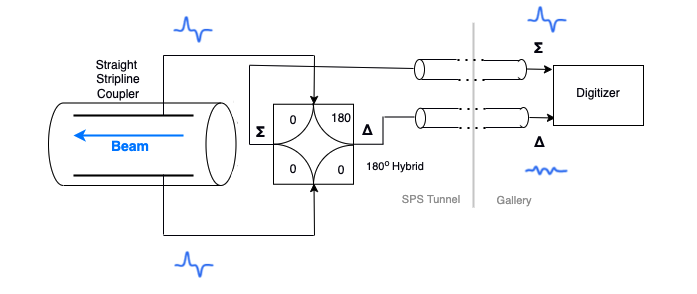
\includegraphics[width=1.0\textwidth]{images/Ch4/HT_monitor_sketch.png}
       \caption{Diagram of the SPS HT monitor~\cite{Levens:2313358}. The beam is passing through a straight stripline coupler which is followed by a 180$^\circ$hybrid. This configuration provides the sum ($\Sigma$) and the difference ($\Delta$) signal of the two electrodes.} %, which correspond to the longitudinal line density and intra-bunch offset, respectively.} 
       \label{fig:SPS_HT_diagram}
\end{figure}
% what is a 180 hybrid. A 180° Hybrid Coupler is a four port device that is used either to equally split an input signal with a 180° phase shift between the ports or to combine two signals that are 180° apart in phase. (from google)

The raw signals from the HT monitor require a specific post-processing procedure~\cite{Levens:2313358}, in order to provide useful information. Figure~\ref{fig:HT_example_signals} shows some example signals obtained from the HT monitor after the basic post-processing is applied. Moreover, Fig.~\ref{fig:HT_example_signals_2D} shows a 2D representation of the HT monitor reading. It is worth noting here that in the specific example a clear modulating pattern in time of the vertical intra-bunch offset (vertical $\Delta$) signal is observed. This is a result of the phase slip between the $\CC$ and the main RF system because they are not yet synchronised. 
% COMMENT: The Ref.~\cite{Levens:2313358} refers to the LHC HT monitor but the same applies for SPS as it is the same device.

\begin{figure}[!h]
   \centering         
   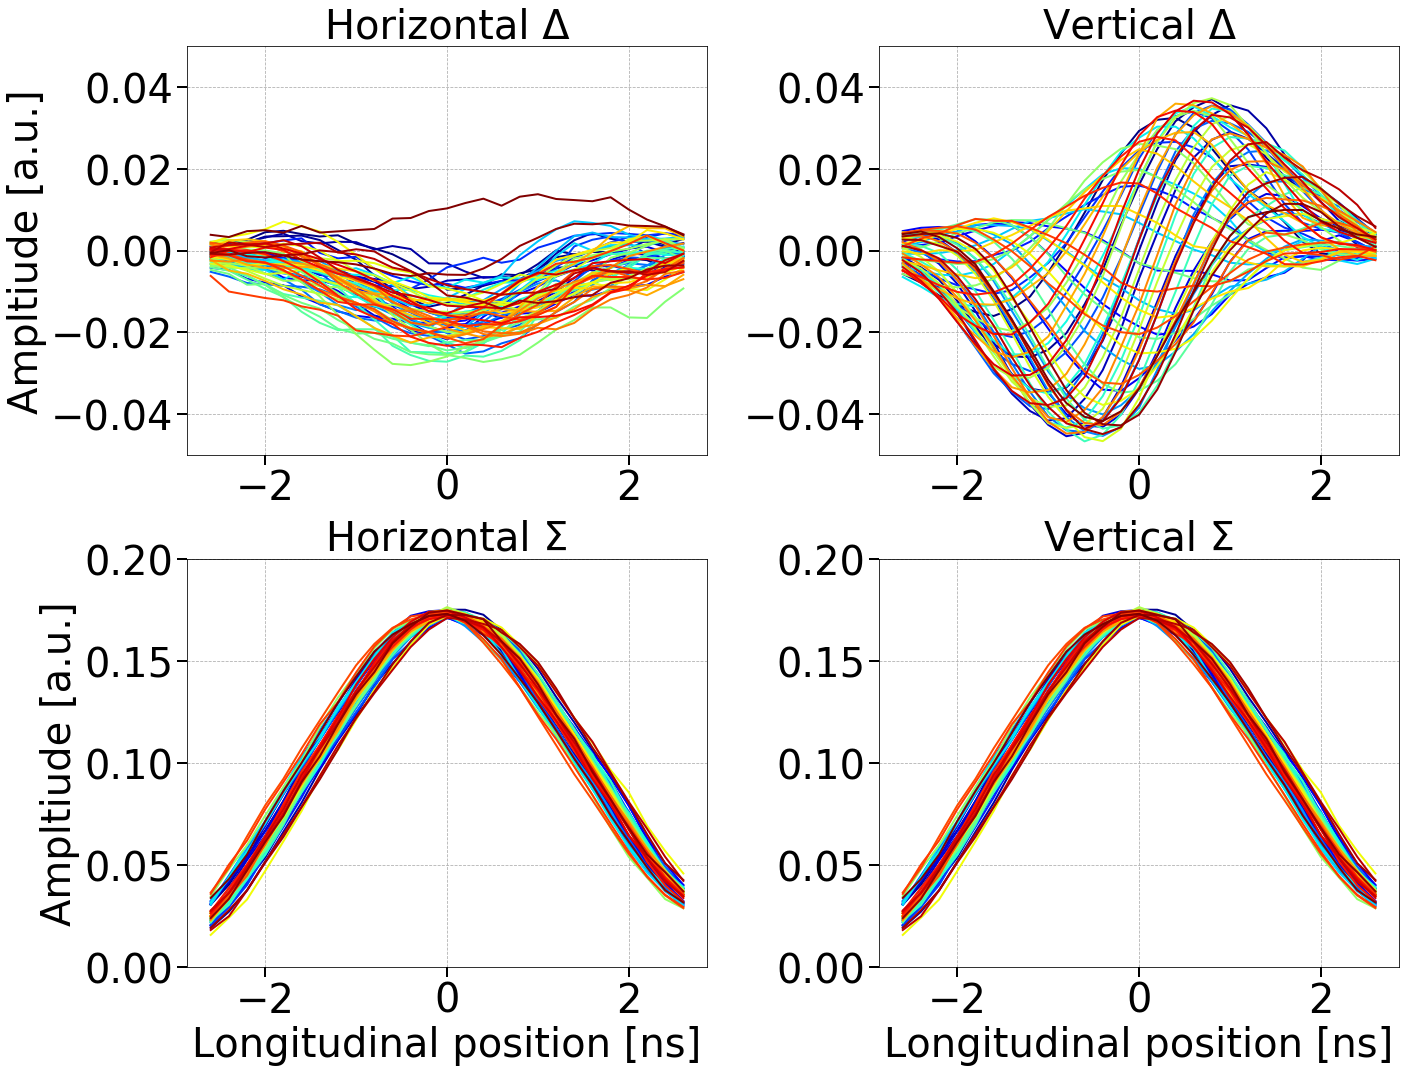
\includegraphics[width=0.8\textwidth]{images/Ch4/HT_1D__20180530_135105exampleAcq_4thesis_turnsStart0_Stop6000_step100_new.png}
       \caption{Example difference and sum signals (top and bottom plots, respectively) from the HT monitor, in time scale, with respect to the longitudinal position within the bunch over several SPS revolutions, after the basic post processing~\cite{Levens:2313358} but before the baseline correction. The different colors indicate the signals from different turns (every 100 turns). } % mention every how many turns you plot, shows an indication of how fast is the instrument.
       \label{fig:HT_example_signals}
\end{figure}
% /eos/user/n/natriant/2018/CC_MD_2018_summary/2018_HT_monitor/MD2_phase_scan_CC1/main_example_135105/plot_1example_HT_acquisition_for_thesis_30May2018-135105_for_thesis_sin_fit_forCh4_fixed_fcc_standard_post_processing_Ch4_3_1.ipynb


\begin{figure}[!h]
   \centering         
   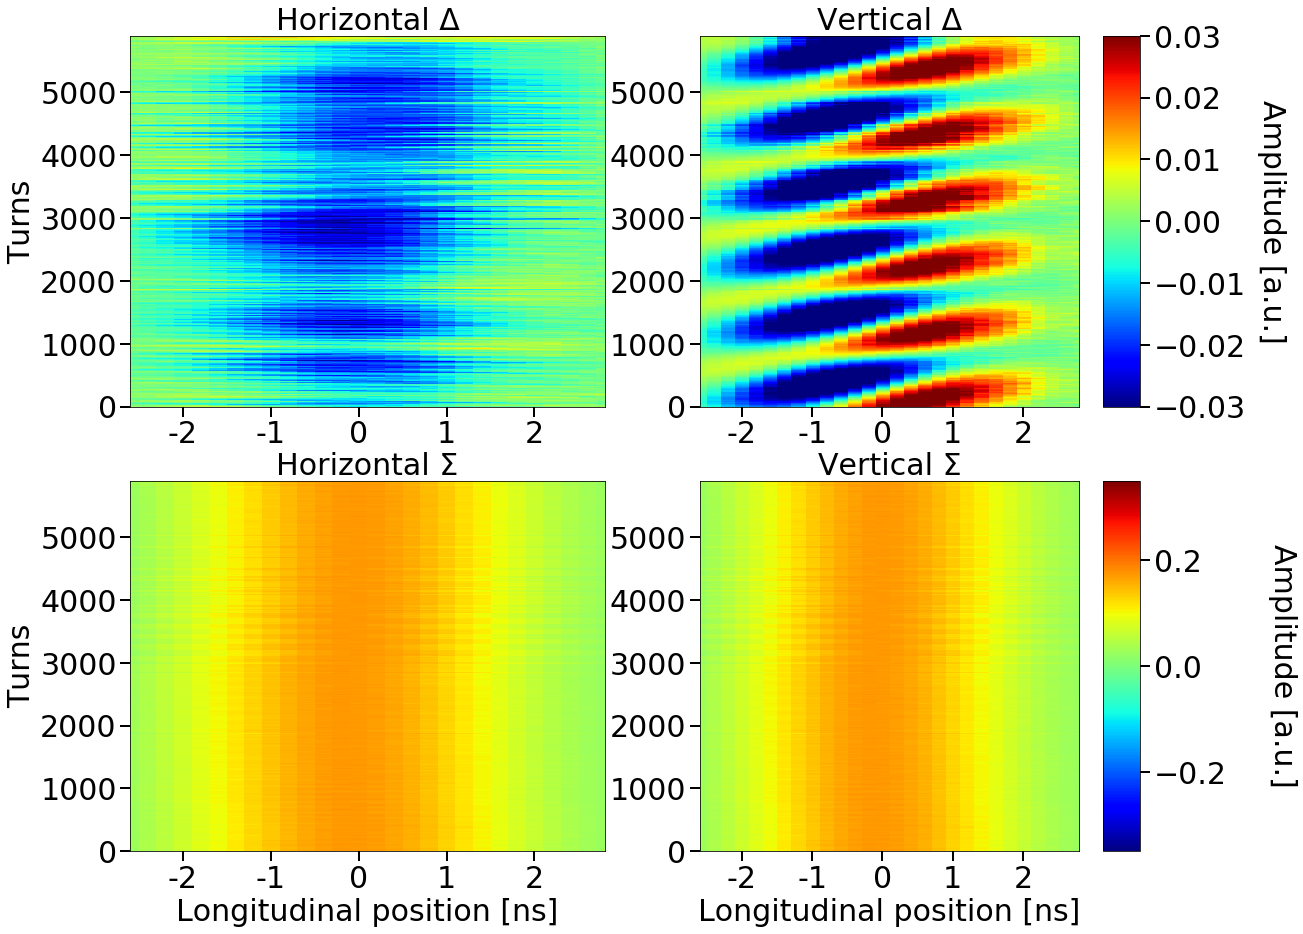
\includegraphics[width=0.9\textwidth]{images/Ch4/HT_2D__20180530_135105_colorbar_new_version.png}
       \caption{2D representation of example difference and sum signals with respect to the longitudinal position within the bunch obtained from the HT monitor over several SPS revolutions.}
       \label{fig:HT_example_signals_2D}
\end{figure}
% /eos/user/n/natriant/2018/CC_MD_2018_summary/2018_HT_monitor/MD2_phase_scan_CC1/main_example_135105/plot_1example_HT_acquisition_for_thesis_30May2018-135105_for_thesis_sin_fit_forCh4_fixed_fcc_standard_post_processing_Ch4_3_1.ipynb

\subsection{Post processing in the presence of Crab Cavities}\label{subsec:HT_post_process_CC}
To obtain useful information from the HT monitor signal in the presence of the $\CC$s there are a few steps that differ from the standard post processing procedure and they are desribed below.

\normalsize{\textbf{Head-Tail monitor baseline correction}}\\
The HT monitor measurement has a baseline on the difference signal which needs to be removed. The baseline is a result of orbit offsets and non-linearities of the instrument and is constant from turn to turn~\cite{Levens:2313358}. Therefore, during the normal post processing procedure (without $\CC$s), the baseline is computed as the mean of the difference signals over all turns and then the correction is achieved by subtracting this static offset from the signal of each turn. However, in the SPS tests, where the $\CC$s are well synchronised with the main RF system (Section~\ref{sec:CC_operational_considerations}), the crabbing signal is also a static intra-bunch position offset and thus would also be removed with the usual method. Because of technical limitations it was not feasible to switch off the $\CC$ for those kind of measurements. Thus, the following technique was used. 
% CC effect average out over time

For the $\CC$ experiments a reference measurement had first to be made with the $\CC$ not being synchronous with the main RF system. The baseline was computed as the mean of the difference signals over this reference period and subsequently it was subtracted from the average of the difference signals acquired after the synchronisation (Fig~\ref{fig:HT_baseline_correction}). The datasets before and after synchronisation are easily distinguishable in the 2D HT monitor reading as displayed in Fig.~\ref{fig:HT_baseline_correction_measurements_2D}

% /eos/user/n/natriant/2018/CC_MD_2018_summary/2018_HT_monitor/MD2_phase_scan_CC1/main_example_135105/plot_1example_HT_acquisition_for_thesis_30May2018-135105_for_thesis_sin_fit_forCh4_fixed_fcc-CC_post_processing_Ch4_3_2_and_after.ipynb
\begin{figure}[!h]
   \centering         
   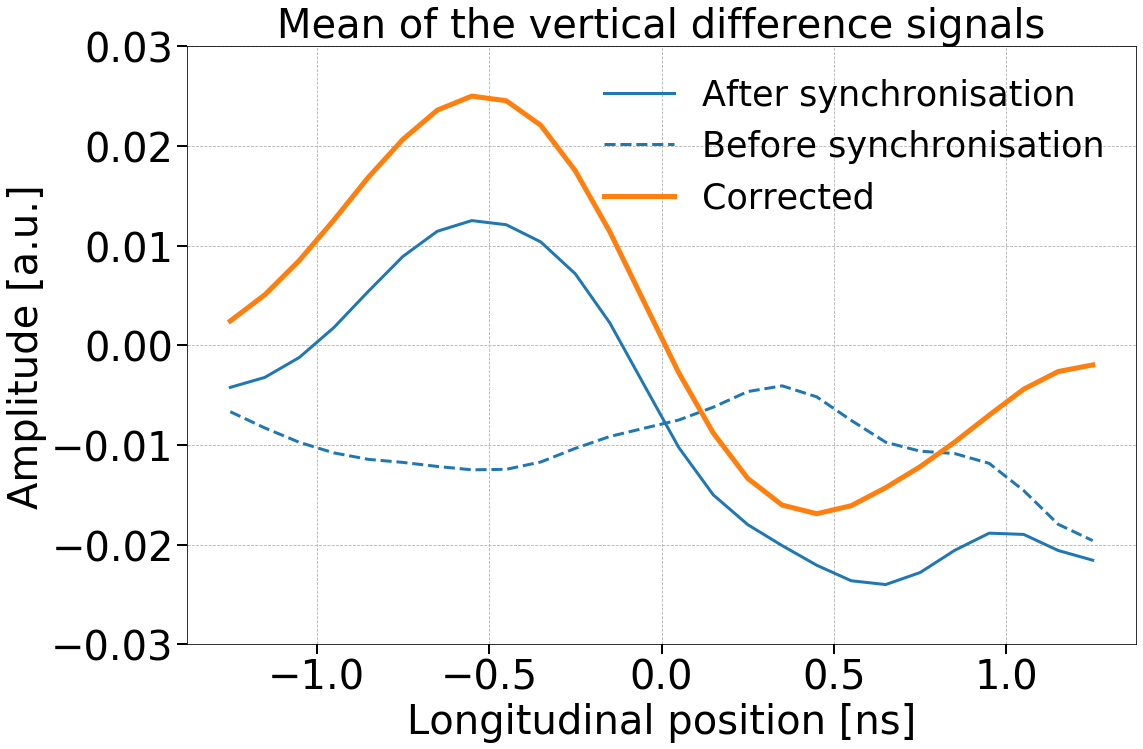
\includegraphics[width=0.65\textwidth]{images/Ch4/HT_measures_vs_reference_vs_corrected__20180530_135105_baseline_correction_new_version_CC_post_processing.png}
       \caption{HT monitor baseline correction for the SPS CC tests. The baseline signal (blue dashed line) refers to the mean of the difference signals acquired before the CC - main RF synchronisation. The measured signal (blue solid line) corresponds to the mean of the difference signal acquired after the synchronisation. Last, the corrected signal (orange solid line) is obtained after subtracting the baseline from the measured signal.}
       \label{fig:HT_baseline_correction}
\end{figure}

% /eos/user/n/natriant/2018/CC_MD_2018_summary/2018_HT_monitor/MD2_phase_scan_CC1/main_example_135105/plot_1example_HT_acquisition_for_thesis_30May2018-135105_for_thesis_sin_fit_forCh4_fixed_fcc_standard_post_processing_Ch4_3_1.ipynb
\begin{figure}[!h]
   \centering         
   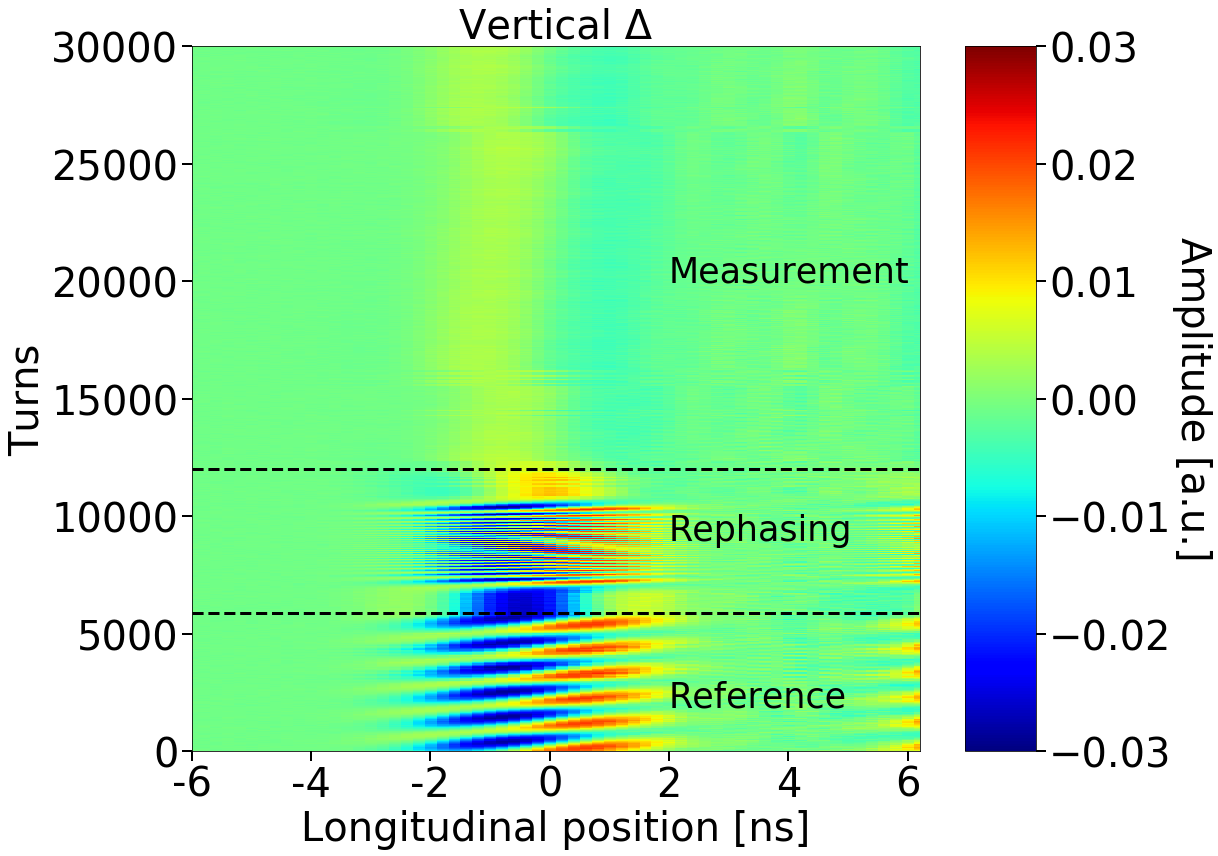
\includegraphics[width=0.7\textwidth]{images/Ch4/HT_2D__20180530_135105_before_after_sunchronisation_new_version.png}
       \caption{HT acquistions before and after the synchronisation of the SPS main RF with the CC.}
       \label{fig:HT_baseline_correction_measurements_2D}
\end{figure}

%At this point, it should be mentioned that the baseline (blue dashed line in Fig.~\ref{fig:HT_baseline_correction}) appears to vary with position within the bunch. The origin for this is not yet understood and will have to be addressed in the future to fully understand .... However, here is our working assumption ...

\normalsize{\textbf{Head-Tail monitor scaling}}\\
The last step to make the HT acquisitions meaningful is to convert the measured intra bunch offset (the mean of the difference signals following phase synchronisation and baseline correction) from arbitrary units to millimeters. The scaling is achieved by dividing by the mean of the sum signals (which is a function of the position along the bunch and is calculated for each point individually over many turns) after the synchronisation and with a normalisation factor which is provided by the calibration of the HT monitor~\cite{PhysRevAccelBeams.22.112803}. The normalisation factor for the SPS was measured at 0.1052 in 2018~\cite{HT_calibration_2018}. Figure~\ref{fig:HT_baseline_correction_crabbing_mm} shows the intra-bunch offset from the $\CC$ kick in millimeters and after the baseline correction. 

% /eos/user/n/natriant/2018/CC_MD_2018_summary/2018_HT_monitor/MD2_phase_scan_CC1/main_example_135105/plot_1example_HT_acquisition_for_thesis_30May2018-135105_for_thesis_sin_fit_forCh4_fixed_fcc-CC_post_processing_Ch4_3_2_and_after.ipynb
\begin{figure}[!h]
   \centering         
   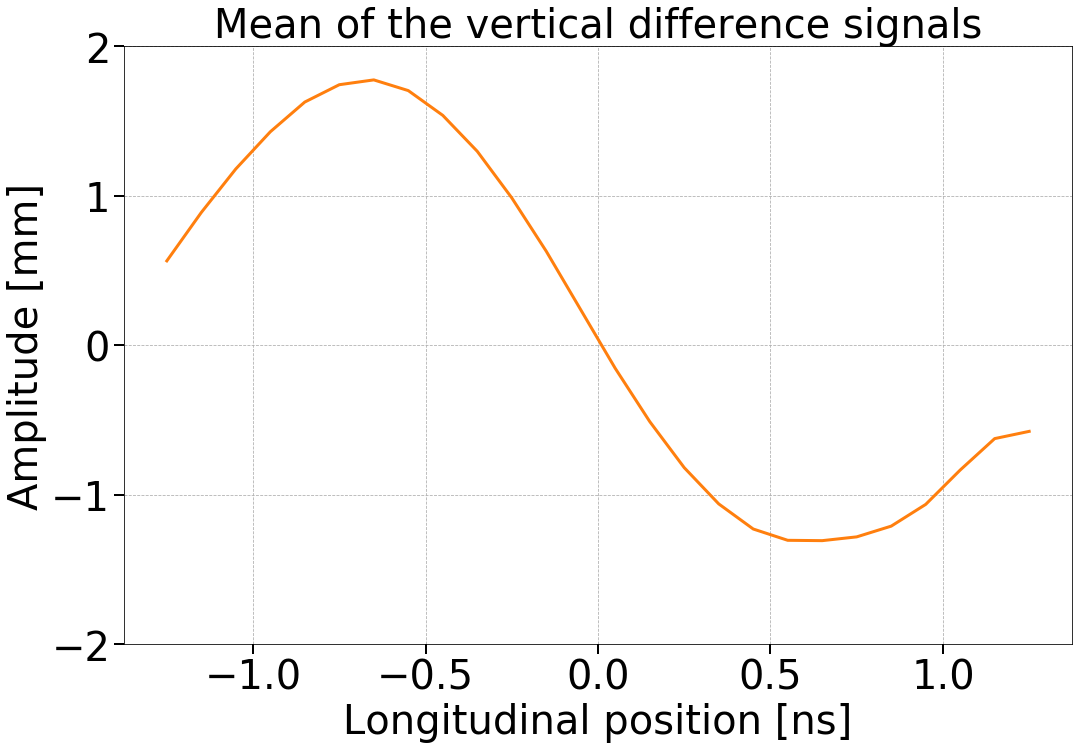
\includegraphics[width=0.65\textwidth]{images/Ch4/HT_corrected__20180530_135105_baseline_correction_new_version_CC_post_processing.png}
       \caption{Intra-bunch offset from the CC kick expressed in millimeters after the removal of the baseline.}
       \label{fig:HT_baseline_correction_crabbing_mm}
\end{figure}


 \subsection{Crab Cavity voltage reconstruction}\label{sec:Vcc_calibration}
 This section discusses the reconstruction of the $\CC$ voltage from the HT monitor signal. First, Eq.~\eqref{eq:CC_orbit_shift_Chao} was used to calculate the $\CC$ kick, $\theta$, required to reconstruct the measured intra-bunch offset. Equation~\eqref{eq:CC_orbit_shift_Chao}, which is obtained from Eq.\,(1) from chapter 4.7.1 in Ref.~\cite{Chao:1490001}, gives the vertical orbit shift (in meters) from the $\CC$ kick, $\theta$, at the HT monitor location as follows:

\begin{equation}\label{eq:CC_orbit_shift_Chao}
   \Delta y_{,HT} = \frac{\sqrt{\beta_{y, HT}}}{2 \sin(\pi \Qy)} \theta \sqrt{\beta_{y, CC}} \cos(\pi \Qy - \mid \psi_{y, HT} - \psi_{y, CC} \mid),
\end{equation}

where $\beta_y$ is the beta function, $\Qy$ is the tune, and $\mid \psi_{y, HT} - \psi_{y, CC} \mid$ is the vertical phase advance (in tune units) between the $\CC$ and the HT monitor. The same applies for the horizontal plane. The subscripts HT and CC indicate quanities at the location of the HT monitor and CC respectively.

The $\CC$ voltage is then reconstructed from the $\CC$ kick which is written as $\theta = - \frac{q V_{CC}(t)}{\symE}$, where $q$ is the charge of the particle, $\symE$ the beam energy and $V_{CC}(t) = \VCC \sin(2 \pi \fCC t + \phiCC) $ is the voltage that a particle experiences while passing through the $\CC$. In the context where the HT monitor measures the signal as a function of time, $t$, the voltage in the above formula is expressed accordingly as $V_{CC}(t)$, where $t=0$ the center of the bunch.

% 1. locally PhD_projects/CC_MD_2021_summary/HT_monitor/2018_HT_monitor/MD2_phase_scan
% /eos/user/n/natriant/2018/CC_MD_2018_summary/2018_HT_monitor/MD2_phase_scan_CC1/main_example_135105/plot_1example_HT_acquisition_for_thesis_30May2018-135105_for_thesis_sin_fit_forCh4_fixed_fcc-CC_post_processing_Ch4_3_2_and_after.ipynb
\begin{figure}[!h]
\centering         
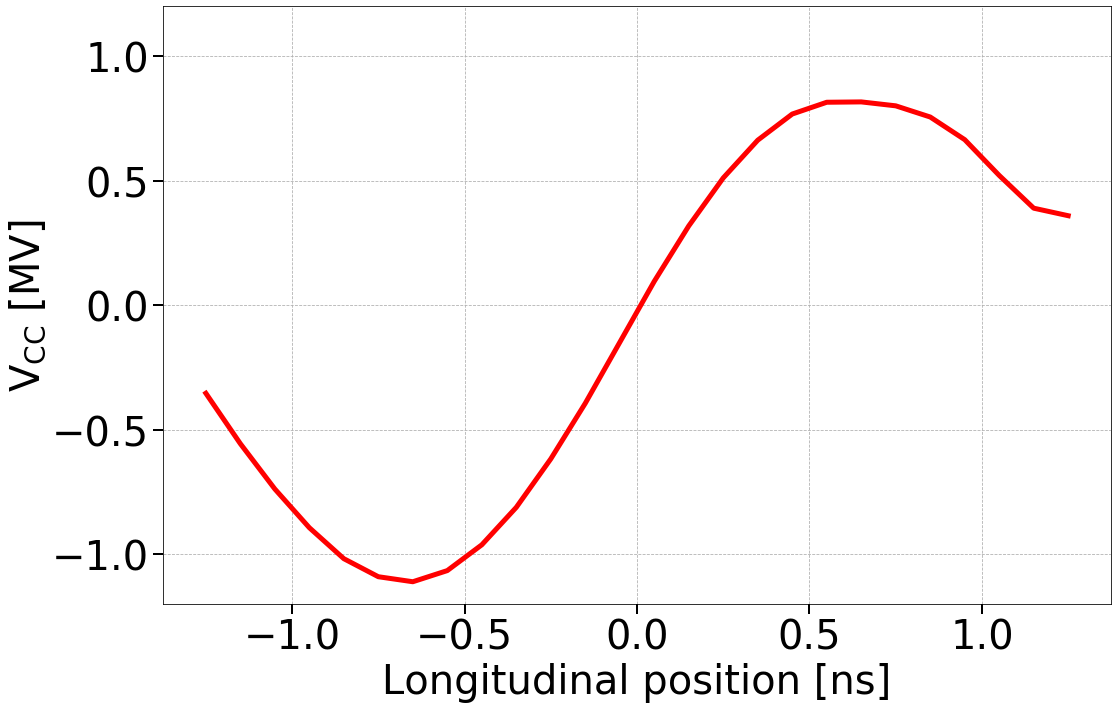
\includegraphics[width=0.65\textwidth]{images/Ch4/HT_VCC_callibration_20180530_135105_CC_post_processing.png}
    \caption{CC voltage reconstruction from the HT monitor.}
    \label{fig:VCC_from_HT_monitor_measurement}
\end{figure}

It should be noted here, that the measured intra-bunch offset, $\Delta y_{, HT}$, is inserted in Eq.~\eqref{eq:CC_orbit_shift_Chao} after removing the baseline and converting it to millimeters as discussed in Section~\ref{subsec:HT_post_process_CC}. Figure~\ref{fig:VCC_from_HT_monitor_measurement} illustrates the cavity voltage computed from the HT signals shown already in this section. The corresponding beam and optic parameters are listed in Table~\ref{tab:SPS_HT_CC}.

% optics at CC1, CC2 and HT monitor location /eos/user/n/natriant/Project_thesis/SPS optics
\begin{table}[!hbt]
	\begin{minipage}{\textwidth}
   \begin{centering}
   \caption{Parameters for computing the CC voltage from the example HT monitor measurements discussed in this chapter.}
	\begin{tabu} to \textwidth {X[c,m] X[0.01c,m] X[0.01c,m] X[0.01c,m]}
		&&& \\[-6mm]
		\toprule \toprule
		\multicolumn{2}{l}{\textbf{Parameter}} &
		\multicolumn{2}{c}{\textbf{Value}} \\
		\bottomrule
      \multicolumn{2}{l}{Beta function at the HT monitor, $\beta_{y, HT}$}& \multicolumn{2}{c}{49.19\,m} \\
      \multicolumn{2}{l}{Phase advance to the HT monitor$^{\ast}$, $\psi_{y, HT}$} & \multicolumn{2}{c}{15.68 $\times$ 2$\mathrm{\pi}$} \\
      \multicolumn{2}{l}{Beta function at the $\CC$1, $\beta_{y, CC1}$}& \multicolumn{2}{c}{76.07\,m} \\
      \multicolumn{2}{l}{Phase advance to the $\CC$1$^{\ast}$, $\psi_{y, CC1}$} & \multicolumn{2}{c}{23.9 $\times$ 2$\mathrm{\pi}$} \\
      \multicolumn{2}{l}{Vertical betatron tune, $\Qy$} & \multicolumn{2}{c}{26.18} \\
      \multicolumn{2}{l}{Beam energy, $\symE$} & \multicolumn{2}{c}{26\,GeV} \\
      \bottomrule
	\end{tabu}
   \label{tab:SPS_HT_CC}
   \end{centering} \footnotesize{$^\ast$ The phase advances are measured from the start of the lattice which is considered the element QF.10010 that is a focusing quadrupole.}
   \end{minipage}
\end{table}

\subsection{Demonstration of crabbing with proton beams}\label{subsec:crabbing_demonstration_density_plot}
Additionally, the measurements from the HT monitor were used for reconstructing the crabbing and representating schematically the beam projection in the transverse plane. The technique for reconstructing the crabbing was developed at CERN in 2018 and was extensively used throughout the experimental campaign with $\CC$s since (together with the calibrated voltage) it gives a straightforward estimate of the applied $\CC$ kick, as illustrated in Fig.~\ref{fig:crabbing_reconstruction_HT_monitor}. 

To obtain this schematic representation, which in practice is a density plot showing the effect of the $\CC$ kick on the beam, one needs to multiply the measured longitudinal profile (the mean of the sum signals acquired after phase synchronisation) with the measured intra-bunch offset, mean of the difference signals acquired after the synchronisation. An example of this is shown in Fig.~\ref{fig:HT_baseline_correction_crabbing_mm}. For the transverse plane a gaussian distribution is considered with $\sigma$ obtained from the wire scanner (addressed in more detail in the following section). The color code of Fig.~\ref{fig:crabbing_reconstruction_HT_monitor} is normalised to the maximum intensity within the bunch.

% /eos/user/n/natriant/2018/CC_MD_2018_summary/2018_HT_monitor/MD2_phase_scan_CC1/main_example_135105/plot_1example_HT_acquisition_for_thesis_30May2018-135105_for_thesis_sin_fit_forCh4_fixed_fcc-CC_post_processing_Ch4_3_2_and_after.ipynb
\begin{figure}[!h]
   \centering         
   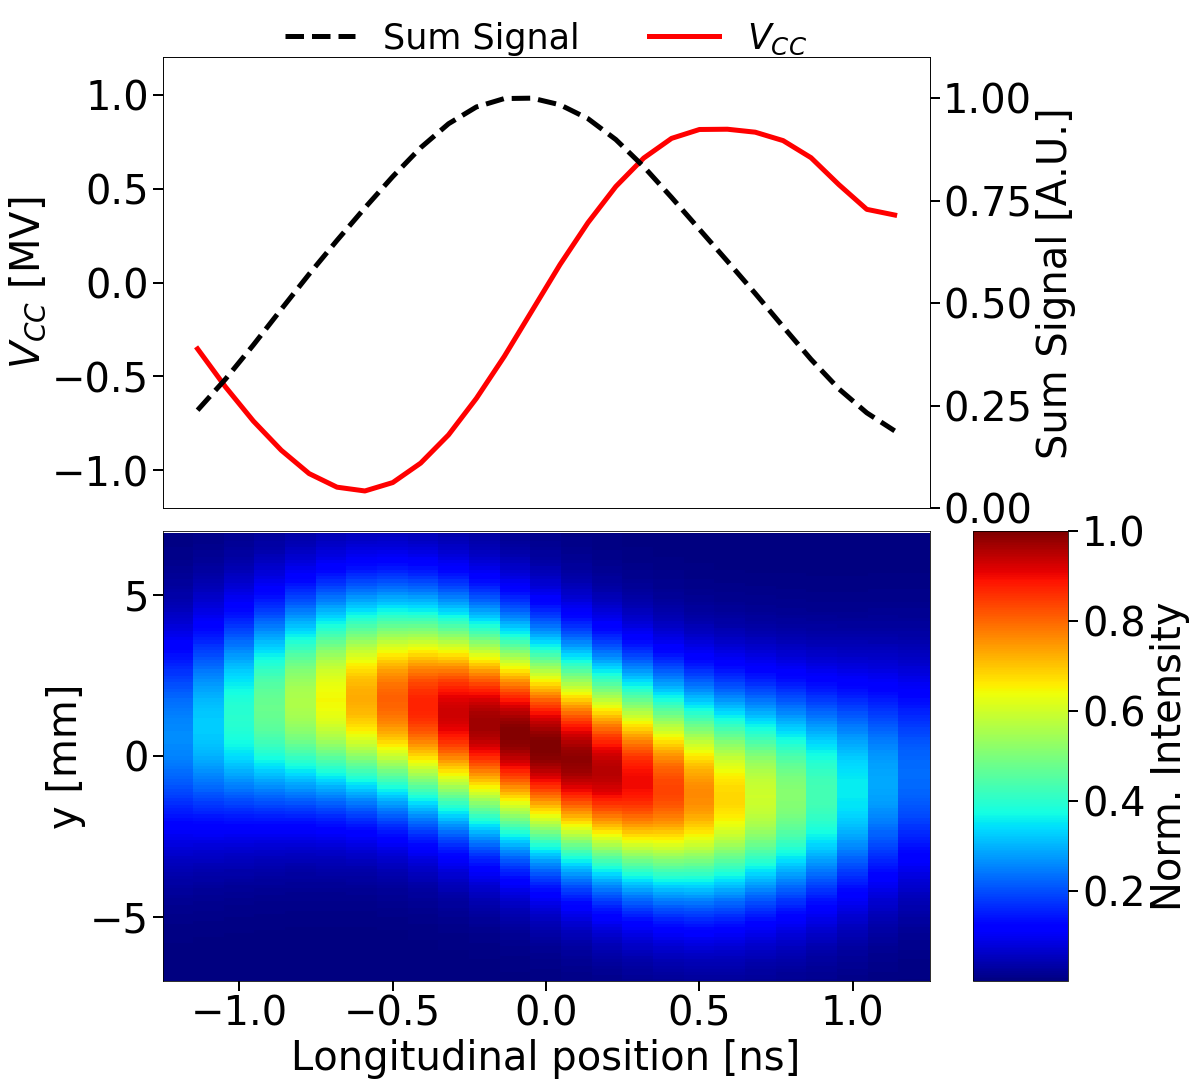
\includegraphics[width=0.7\textwidth]{images/Ch4/HT_crabVoltage__20180530_135105_crabbing_only_CC_post_processing.png}
       \caption{Demonstration of the crabbing from the HT monitor signal. CC voltage and sum signal (longitudinal line density) measured from the HT monitor (top) together with the density plot (bottom) which visualises the effect of the CC kick on the beam.}
       \label{fig:crabbing_reconstruction_HT_monitor}
\end{figure}
   

\section{Characterisation of measured Crab Cavity voltage}\label{sec:CC_voltage_meas}
This section gives the definitions of the amplitude of the beam-based measurement of the $\CC$ voltage and its uncertainty that will be used in this thesis. Additionally, their dependence on the $\CC$ phase is discussed for completeness.

\subsection{Definitions of the amplitude and the uncertainty of the measurement}\label{subsec:def_amplt_uncertainty}
The voltage amplitude, $\VCC$, is obtained from a sinusoidal fit on the reconstructed voltage, $\VCC (t)$, from the HT monitor reading. The standard procedure of least squares fitting (see Appendix section~\ref{app:non_linear_fitting}) is followed. In particular, $\VCC (t)$ is fitted with the folllowing three-parameter ($\VCC$, $\phiCC$, $k$) model function which also provides the $\CC$ phase and voltage offset:
\begin{equation}\label{eq:sin_fit_cc}
   f(x) = V_{CC}\sin{(2\pi \fCC x + \phiCC)} + k ,
\end{equation}

where $\VCC$ is the amplitude of the $\CC$ voltage, $\phiCC$ the $\CC$ phase and
$k$ the voltage offset. The fit is performed for a fixed $\CC$ frequency, as the operational value is well known and in particular it equals, $\fCC$=400.78\,MHz. The offset parameter is added to the model function as it is clear from Fig.~\ref{fig:VCC_from_HT_monitor_measurement} and~\ref{fig:crabbing_reconstruction_HT_monitor} that the reconstructed $\CC$ voltage, $\VCC(t)$, is not centered around zero. The assymetry seems to be a result of the HT monitor pick up and cable response~\cite{Levens_WP2_HT_CC_diagnostic}. However its origin is not yet fully understood and will have to be addressed in the future. %the assymetry of the reconstructed voltage for this assynetris not yet understood and will have to be addressed in the future to fully understand .... However, here is our working assumption ...

In order to obtain results that correspond to the experimental conditions the following constraints are imposed to the fit. First the voltage amplitude, $\VCC$, is requested to always be positive and higher than 0.7\,MV. Furthermore, the part of the signal that corresponds to the tails of the bunch is excluded from the fit in order not to degrade its quality. Consequently, only the part of the signal for which the corresponding normalised sum signal is above 0.4 is used for the fit. 

Fig.~\ref{fig:crabbing_sin_fit_MD2} shows the result of the fit for the same signal that was analysed in the previous section. As indicated on the top of the plot, the red solid line corresponds to the reconstructed $\CC$ voltage, while the blue solid line corresponds to the result of the sinusoidal fit. It can be seen that only the part of the signal for which the normalised sum signal (black dashed line) is above 0.4 is used. Finally the blue dashed line shows the result of the fit after the voltage offset is subtracted, so that is centered around zero. The parameter values obtained from the fit are given in the legend. Last, the density plot is also shown at the bottom of the figure for a complete visualisation of the crabbing. 

% /eos/user/n/natriant/2018/CC_MD_2018_summary/2018_HT_monitor/MD2_phase_scan_CC1/main_example_135105/plot_1example_HT_acquisition_for_thesis_30May2018-135105_for_thesis_sin_fit_forCh4_fixed_fcc-CC_post_processing_Ch4_3_2_and_after.ipynb
\begin{figure}[!h]
   \centering         
   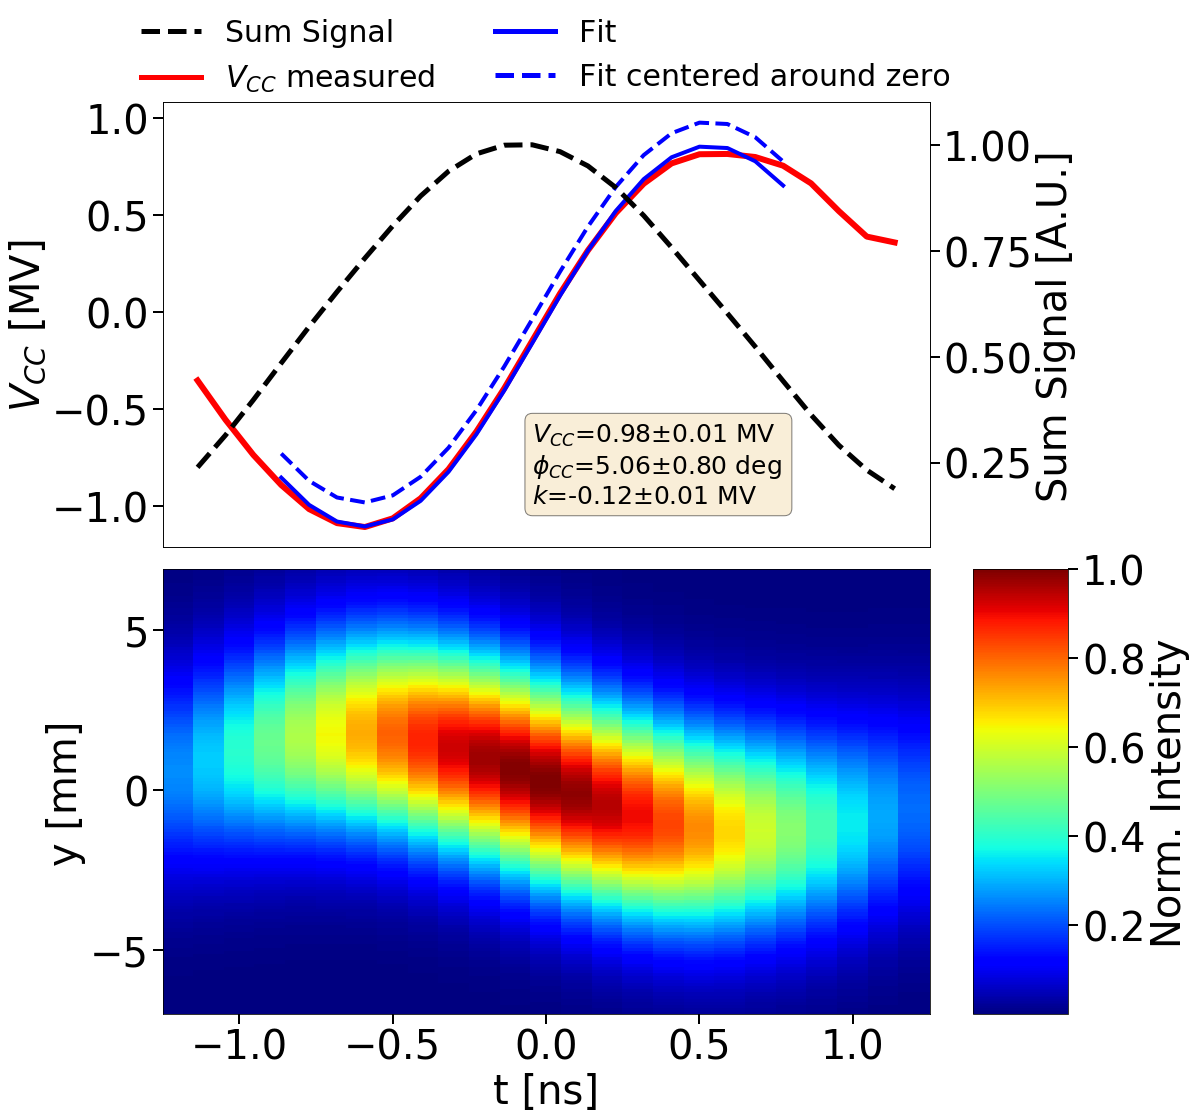
\includegraphics[width=0.7\textwidth]{images/Ch4/HT_VCC_callibration_20180530_135105_sin_fit_fixed_freq_CC_post_processing.png}
       \caption{Demonstration of the sinusoidal fit on the HT monitor reading in order to obtain the CC parameters. A four-parameter sinusoidal fit is performed using Eq.~\eqref{eq:sin_fit_cc} in order to obtain the amplitude, $V_{CC}$, the frequency, $f_{CC}$, the phase, $\phi_{CC}$, and the voltage offset, $k$. The fit results are given in the yellow box.}
       \label{fig:crabbing_sin_fit_MD2}
\end{figure}

In this thesis, the uncertainty on the measured voltage amplitude, $\Delta V_{CC}$ is defined as the absolute value of the voltage offset, $k$, instead of the error of the fit on the voltage amplitude. This is because the voltage offset depicts better the uncertainty of the voltage seen by the beam, $\VCC$. Therefore, for the analyzed example here the $\CC$ voltage was measured to be $\VCC$ = 0.98\,MV and its uncertainty $\Delta V_{CC}$ = 0.12\,MV. 


%- The uncertainty on the Vcc measurement is a systematic uncertainty not statistical/random (like the one I proposed). - What is the value of the CC voltage seeing by the beam during the measurement. What is the uncertainty of the CC voltage seeing by the beam. Is dominated by the systematic error. - Offset, calibration issue with the HT monitor. Limitation of what the instrument can do. -Uncertainty Vcc ~ 10% - - Systematic and random.


\subsection{Dependence of the crab cavity voltage and offset on the phase}

The impact of the $\CC$ phase on the voltage experienced by the beam and on the uncertainty of its measurement was also studied experimentally. Data for the study were collected on 30 May. 2018, at the SPS injection energy of 26\,GeV for a range of different settings of the phase of CC1. The results are summarised in Fig.~\ref{fig:phase_scan_CC1}.

\begin{figure}[!ht]
   \centering
   \begin{subfigure}[t]{0.45\textwidth}
       \centering
       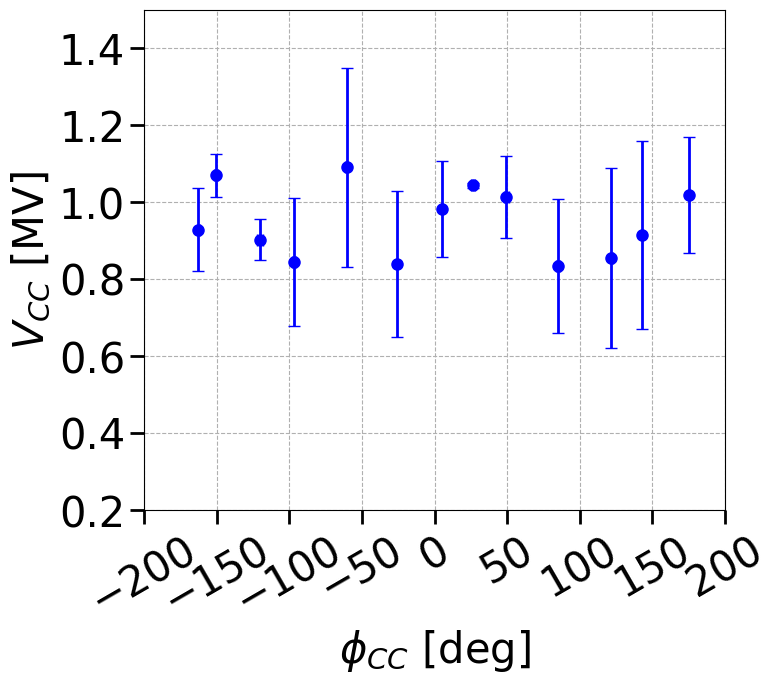
\includegraphics[width=1\textwidth]{images/Ch4/Vcc_vs_phase.png}
       %\caption{$y=\sin(2 \pi f t),\ f=50$ Hz}
       %\label{fig:signal_and_DFT_example_a}
   \end{subfigure}
   \hfill
   \begin{subfigure}[t]{0.45\textwidth}
       \centering
       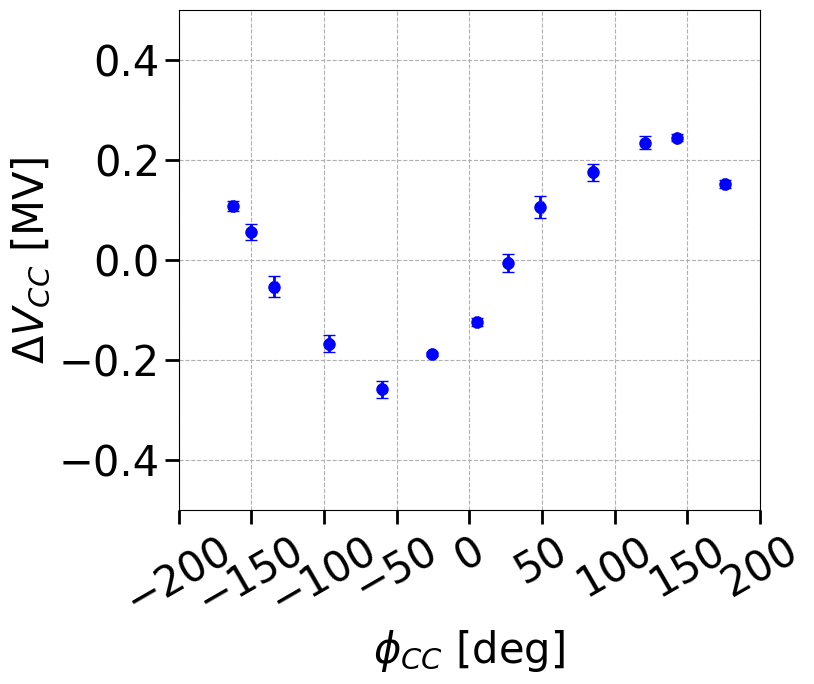
\includegraphics[width=1\textwidth]{images/Ch4/DeltaVcc_vs_phase.png}
       %\caption{Discrete Fourier transform}
       %\label{fig:phase_scan_CC1}
   \end{subfigure}
   \hfill
    \caption{Phase scan with CC1 at 26\, GeV. The sensitivity of the measured CC voltage (left) and its uncertainty (right) on the phase is studied. The error bars of the voltage, $V_{CC}$, indicate the uncertainty, $\Delta V_{CC}$. The error bars of the uncertainty, $\Delta V_{CC}$, and the phase, $\phi_{CC}$, correspond to the error of the respective fit result (see Appendix~\ref{app:non_linear_fitting}) The error bars are not visible here as they are smaller than the markers.
    }
    \label{fig:phase_scan_CC1}
\end{figure}

In the left plot the error bars of the voltage, $V_{CC}$, indicate the uncertainty, $\Delta V_{CC}$. In the right plot, the error bars of the uncertainty, $\Delta V_{CC}$, correspond to the error of the fit result for the $\VCC$ parameter  (see Appendix~\ref{app:non_linear_fitting}). The horizontal error bars in both left and right plots, of the phase, $\phi_{CC}$, correspond to the error of the fit result for the phase parameter (see Appendix~\ref{app:non_linear_fitting}). It should be noted that the error bars of the 
phase values are smaller than the markers and are hence not visible in the plots. 

The phase scan does not reveal any systematic dependence of the measured voltage, $\VCC$, on the phase, as expected. However, there is a variation of the voltage offset, $\Delta \VCC$, with the phase. The origin of this, which seems to be a systematic effect, is not yet understood and will be addressed in the future to fully characterise the behavior of the beam in the presence of a phase offset in the $\CC$. It should be pointed out that the impact of this effect on the interpreting the $\CC$ noise induced emittance growth measurements is limited and thus it will not be a matter of concern for this thesis. 

% Scripts for phase scan: 1. Post process: /eos/user/n/natriant/2018/CC_MD_2018_summary/2018_HT_monitor/MD2_phase_scan/phase_scan/Vcc_iterate_h5_all_sin_fit_selected_with_offset.py, 2. Plot /eos/user/n/natriant/2018/CC_MD_2018_summary/2018_HT_monitor/MD2_phase_scan/phase_scan/plot_Vcc_offset_vs_phase_for_Ch4_thesis.py
